\documentclass[12pt,a4paper]{report}

%###################################################################################
%###################### Document Defintions ########################################
%###################################################################################
%aubrey: no real need to change these
%how to handle spaces
\sloppy
\makeindex

\usepackage[latin1]{inputenc}
\usepackage{amsmath, marvosym} % Mathematik
\usepackage{harvard} %for harvard style citation, keep this position before url package
\usepackage{times, url, geometry, amssymb, booktabs}
\usepackage{hyperref} %Hyperlinks zw. Textstellen
\usepackage[pdftex]{graphicx} %pdf figures
\usepackage{subfig} %multi-figures
\usepackage{listings} %code listings
\usepackage{multirow} %for multi-row tables
\usepackage{color} %needed for listings

\definecolor{Grey}{rgb}{0.83,0.83,0.83}
\definecolor{White}{rgb}{1,1,1}

%\newcommand{\nessi}{\texorpdfstring{\textit{NeSSi\textsuperscript{2}}}{NeSSi 2}}
%\newcommand{\nessiUI}{\nessi{} User Interface}

%\newcommand{\lineFive}[6]{\cellcolor{#1}#2&\cellcolor{#1}#3&\cellcolor{#1}#4&\cellcolor{#1}#5&\cellcolor{#1}#6\\}

%\newcommand{\whiteLineFive}[5]{\lineFive{White}{#1}{#2}{#3}{#4}{#5}}
%\newcommand{\blueLineFive}[5]{\lineFive{Grey}{#1}{#2}{#3}{#4}{#5}}


%depth of section
\setcounter{secnumdepth}{4}
%depth of TOC
\setcounter{tocdepth}{3} 
%directory for graphics
\graphicspath{{gfx/}}

%setting for listing
\lstset{
	extendedchars=true,
	basicstyle=\scriptsize\ttfamily,
	%basicstyle=\tiny\ttfamily,
	tabsize=2,
	keywordstyle=\textbf,
	commentstyle=\color{grau},
	stringstyle=\textit,
	numbers=left,
	numberstyle=\tiny,
	% f�r sch�nen Zeilenumbruch
	breakautoindent  = true,
	breakindent      = 2em,
	breaklines       = true,
	postbreak        = ,
	%prebreak         = \raisebox{-.8ex}[0ex][0ex]{\ensuremath{\lrcorner}},
	prebreak         = \raisebox{-.8ex}[0ex][0ex]{\Righttorque},
}

%Table of Content TOC settings
\setcounter{tocdepth}{3}
%This is needed for entering URLs for harvard citation style
\renewcommand{\harvardurl}{URL: \url}


%###################################################################################
%########################### Thesis content ########################################
%###################################################################################
\begin{document}
%__________________________Start_of_Thesis______________________________________________
%Roman numeral numbering for initial section of thesis
\pagenumbering{roman}
%title page specification, deployed as seperate file the input folder
%############################################################################
%########################### Change This ####################################
%############################################################################
%put your title here
\newcommand{\trtitle}{Problem Set 4: Support Vector Machines}
%replace with "Bachelor Thesis", "Master Thesis" or "Diplomarbeit"
\newcommand{\trtype}{Report Machine Learning Lab Course}
%your name
\newcommand{\trauthor}{Budi Yanto}
% your matrikelnummer
\newcommand{\trmatrikelnummer}{308819}
\newcommand{\tremail}{budiyanto@mailbox.tu-berlin.de}
%supevisor
%\newcommand{\trbetreuerA}{Daniel Bratz}
%\newcommand{\trbetreuerB}{Dipl.-Ing. Jo\"{e}l Chinnow}
%estimator 1
\newcommand{\trguta}{Daniel Bartz}
%estimator two
\newcommand{\trgutb}{Felix Brockherde}
\newcommand{\trdate}{\today}

%############################################################################
%########################### DO NOT touch this, unless you need to ##########
%############################################################################
\thispagestyle{empty}
%head line logo + tub + logo
\begin{tabular}{lcc}
\includegraphics[width=0.15\textwidth]{template/TUBerlin_Logo_rot_hell}& \hspace{1.1cm} Technische Universit{\"a}t Berlin& \hspace{1.2cm} 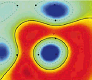
\includegraphics[width=0.15\textwidth]{template/ml_logo}\\
\end{tabular}
%draw a line
\rule{\textwidth}{0.4pt}
%aub: remove this on final submission
%\begin{center}
%DOCUMENT BUILD DATE: \today\\%
%add your status here, e.g. First Draft for Supervizor etc.
%DOCUMENT STATUS: Beta
%\end{center}

%vertical space
\vspace{2.5cm}
\begin{center}
%replace this
  \textbf{\LARGE \trtitle}
\end{center}
\vspace{2cm}

\begin{center}
  \textbf{\trtype} \\
  Fachgebiet Maschinelles Lernen\\
  Prof.\ Dr.\ Klaus-Robert M�ller \\
  Fakult�t IV Elektrotechnik und Informatik \\
  Technische Universit�t Berlin \\[0.5cm]
  submitted by \\
  \textbf{\trauthor}
\end{center}

\vspace{1cm}


\begin{center}
\begin{tabular}{ll}
Instructor:& \trguta\\
& \trgutb\\
\end{tabular}
\end{center}

\vfill

\begin{tabular}{l}
Matrikelnummer:  \trmatrikelnummer \\
Email: \tremail \\
\end{tabular}

\rule{\textwidth}{0.4pt}

\clearpage
%abstract plus acknowledgement and statement
%%#############################################################
%###################### Statement ############################
%#############################################################
\chapter*{Erkl{\"a}rung der Urheberschaft}
%this one needs to be signed for submission
Ich erkl�re hiermit an Eides statt, dass ich die vorliegende Arbeit ohne Hilfe Dritter und ohne Benutzung anderer als der angegebenen Hilfsmittel angefertigt habe; die aus fremden Quellen direkt oder indirekt �bernommenen Gedanken sind als solche kenntlich gemacht. Die Arbeit wurde bisher in gleicher oder �hnlicher Form in keiner anderen Pr�fungsbeh�rde vorgelegt und auch noch nicht ver�ffentlicht.


\vspace{4cm}

Berlin, 12 December 2012 \hfill Signature

%#############################################################
%###################### Abstract  ############################
%#############################################################
\newpage



\chapter*{Abstract}

\textbf{Deutsch und Englisch}

%DELETEME: An abstract is a teaser for your work. You try to convince a reader that it is worth reading your work. Normally, it makes to structure you abstract in this way: 
%\begin{itemize}
%\item one paragraph on the motivation to your topic
%\item one paragraph on what approach you have chosen
%\item and one paragraph on your results which may be presented in comparison to other approaches that try to solve the same or a similar problem.
%\end{itemize}
%Abstract should not exceed one page (aubrey's opinion)

%#############################################################
%###################### German Abstract ######################
%#############################################################
\newpage
\chapter*{Conclusion}
DELETEME: translate to German to Englisch or vice-versa.

%#############################################################
%###################### Acknowledgements #####################
%#############################################################
\newpage
\chapter*{Acknowledgements}
DELETEME: Thank you for the music, the songs I am singing
%TOC
\tableofcontents
%add list of figures to TOC
\cleardoublepage
\addcontentsline{toc}{chapter}{List of Figures}
\newpage
\listoffigures
%add list of tables to TOC
\cleardoublepage
\addcontentsline{toc}{chapter}{List of Tables}
\newpage
\listoftables

%__________________________Main_Content______________________________________________
\newpage
%from now on, numbering should be arabic
\pagenumbering{arabic}
\chapter{Implementation}
\label{implementation}
%#############################################################################################
%######################           Motivation          ########################################
%#############################################################################################

This chapter explains the implementation of some algorithms that we will use in this problem set. It includes: \textit{PCA}, \textit{$\gamma$-index} and \textit{LLE}.

\section{Assignment 1: PCA}
\label{sec:assignment1}

In this assignment we have to implement the function \textit{pca} which receives a \textit{d x n} matrix \textit{X} and the number of components \textit{m} as parameters, and returns the principal components as well as the projected data points in a \textit{m x n} matrix \textit{Z}. Furthermore, the function should also return a \textit{d x d} matrix \textit{U} and a \textit{1 x d} vector \textit{D}. The matrix \textit{U} contains the principal directions, whereas the vector \textit{D} contains the principal values, sorted in descending order ($D_1 \geq D_2 ...$).

I have tested the implemented function on the test data and it passed the test. Following steps are performed in the function:
\begin{enumerate}
	\item Substract \textit{X} from its mean.
	\item Calculate the covariance matrix from zero-mean \textit{X}.
	\item Calculate the eigenvectors and eigenvalues from the covariance matrix.
	\item Sort the eigenvalues and eigenvectors in decending order.
	\item Form the feature vectors by taking only the first \textit{m} eigenvectors.
	\item Project the zero-mean \textit{X} to the feature vectors.
\end{enumerate}

%######################################################################################
\section{Assignment 2: $\gamma$-Index}
\label{sec:assignment2}

The $\gamma$-index has to be implemented in this assignment. The function receives a \textit{d x n} matrix \textit{X} containing the data points and the numbers of neighbours \textit{k}, and returns the $\gamma$-index for each data points in the \textit{1 x n} vector \textit{y}.

\citeasnoun**{Harmeling2006} formulate the the formula to calculate the $\gamma$-index for one data point as follows:
$\gamma(x)=\frac{1}{k} \sum_{j=1}^{k} \| x-z_j(x) \|$

The implemented function has passed the test. Following steps are performed in the function:
\begin{enumerate}
	\item Implement a new function \textit{distmat} that calculates the distances from the data points to each other and return the distances as a matrix.
	\item Get the distance matrix using the function \textit{distmat} mentioned above.
	\item Sort the distance matrix in ascending order.
	\item Take only the \textit{k}-nearest data points as neighbours for each data point.
	\item Calculate the mean from the distances of the \textit{k}-nearest neighbours and set it as the $\gamma$-index.
	
\end{enumerate}


%######################################################################################
\section{Assignment 3: LLE}
\label{sec:assignment3}

The last assignment in the implementation part asks us to implement the \textit{locally linear embedding} method as described in \cite{Saul2000}. The \textit{lle} function returns a \textit{m x n} matrix \textit{Y} representing the resulting embedding and takes following parameters as inputs:
\begin{itemize}
	\item A \textit{d x n} matrix \textit{X} containing the data points.
	\item A scalar \textit{m} representing the dimension of the resulting embedding.
	\item A string \textit{n\_rule} determining the method (\textit{'knn'} or \textit{'eps-ball'}) for building the neighbourhood graph.
	\item A scalar \textit{param} used as parameter for the \textit{n\_rule} (\textit{k} or $\epsilon$, respectively).
	\item A scalar \textit{tol} determining the size of the regularization parameter.
\end{itemize}

The implementation is based on the pseudocode described by \citeasnoun{Roweis} on their website, which contains of three main parts:
\begin{enumerate}
	\item Find the nearest neighbours of each data point based on \textit{n\_rule}.
	\item Solve for reconstruction weights \textit{W}.
	\item Compute embedding coordinates \textit{Y} using weights \textit{W}.
\end{enumerate}

\chapter{Application}
\label{application}
%#############################################################################################

In this chapter, we are trying to apply the algorithms that are described and implemented in~\ref{implementation} to various datasets: \textit{usps}, \textit{banana}, \textit{fishbowl}, \textit{swissroll} and \textit{flatroll}.

\section{Assignment 4: PCA}
\label{assignment4}

This assignment askes us to apply \textit{PCA} to the \textit{usps} data set and visualizing the results. The \textit{usps} dataset consists of images of digit zero to nine, and each digit can be viewed as a class. Firstly, i seperate the data set according to each digit into ten classses and then applied \textit{PCA} to each class. The \textit{PCA} was applied to the original data set and noisy data set.

\subsection{Original Data Set}
\label{ass4:original}

The original data set contains of 2007 images and each image has a dimension of \textit{16 x 16}. 

\subsection{Noisy Data Set}
\label{ass4:noisy}



%#############################################################################################

\section{Assignment 5: Outlier Detection Using $\gamma$-Index}
\label{assignment5}

%#############################################################################################

\section{Assignment 6: LLE}
\label{assignment6}

%#############################################################################################

\section{Assignment 7: LLE With Noise}
\label{assignment7}
\chapter{Backend Integration}
\label{mainone}

\section{Problems}
    



%DELETEME: In this chapter you start addressing your actual problem. Therefore, it makes often sense to make a detailed problem analysis first (if not done in introduction). You should be sure about what to do and how. As writtin in the background part, it might also make sense to include complex background information or papers you are basing on in this analysis. If you are solving a software problem, you should follow the state of the art of software development which basically includes: problem analysis, design, implementation, testing, and deployment. Maintenance is often also described but I believe this will not be required for most theses. Code should be placed in the appendix unless it is solving an essential aspect of your work.

 
\chapter{Frontend Integration}
\label{maintwo}


\chapter{Agent Framework Integration}
\label{mainthree}

\section{Problems}
    Yet to be implemented
\section{Solutions}
    Yet to be implemented
\section{Summary}
    
\chapter{Evaluation}
\label{evaluation}
DELETEME: The evaluation chapter is one of the most important chapters of your work. Here, you will prove usability/efficiency of your approach by presenting and interpreting your results. You should discuss your results and interprete them, if possible. Drawing conclusions on the results will be one important point that your estimators will refer to when grading your work.


\chapter{Conclusion and Future Work}
\label{conclusion}
%#############################################################
%###################### Summary   ############################
%#############################################################
\section{Summary}
    Summarize from Chapter 2 to Chapter 6
%DELETEME: put a plain summary of your work here. Summaries should be made of each Chapter beginning with Chapter~2 and ending with you evaluation. Just write down what you did and describe the corresponding results without reflecting on them.

%#############################################################
%###################### Conclusion ###########################
%#############################################################
\section{Conclusion}
    \subsection{Good points}
    \subsection{Drawbacks}
%DELETEME: do not summarize here. Reflect on the results that you have achieved. What might be the reasons and meanings of these? Did you make improvements in comparison to the state of the art? What are the good points about your results and work? What are the drawbacks? 


%__________________________End_of_Thesis______________________________________________
\cleardoublepage
\addcontentsline{toc}{chapter}{Bibliography}
%harvard citations style, please uncomment harvard package in the usepackage area
\bibliographystyle{agsm}
%remove the following line when using harvard style citation
%\bibliographystyle{plain}
%specify bibtex file here
\bibliography{input/mybib}
%add appendix to TOC
\addcontentsline{toc}{chapter}{Appendices}
\chapter*{Appendices}
\label{appendices}
DELETEME: everything that does not fit into your work, e.g. a 5 page table that breaks the reading flow, should be placed here

%###################################################################################
%###################### Appendix A          ########################################
%###################################################################################
%uncomment, if desired
%\newpage
\addcontentsline{toc}{section}{Appendix A: Abbreviations}
\section*{Appendix A: Abbreviations}
\begin{center}
\begin{tabular}{ll}
\textbf{AES}	&	Advanced Encryption Standard (Symmetrisches Verschl�sselungsverfahren)\\
\textbf{ASCII}&	American Standard Code for Information Interchange (Computer-Textstandard)\\
\textbf{dpi}	&	dots per intch (Punkte pro Zoll; Ma� f�r Aufl�sung von Bilddateien)\\
\textbf{HTML}	&	Hypertext Markup Language (Textbasierte Webbeschreibungssprache)\\
\textbf{JAP}	&	Java Anon Proxy\\
\textbf{JPEG}	&	Joint Photographic Experts Group (Grafikformat)\\
\textbf{JPG}	&	Joint Photographic Experts Group (Grafikformat; Kurzform)\\
\textbf{LED}	&	Light Emitting Diode (lichtemittierende Diode)\\
\textbf{LSB}	&	Least Significant Bit\\
\textbf{MD5}	& Message Digest (Kryptographisches Fingerabdruckverfahren)\\
\textbf{MPEG}	&	Moving Picture Experts Group (Video- einschlie�lich Audiokompression)\\
\textbf{MP3}	&	MPEG-1 Audio Layer 3 (Audiokompressionformat)\\
\textbf{PACS}	&	Picture Archiving and Communication Systems\\
\textbf{PNG}	&	Portable Network Graphics (Grafikformat)\\
\textbf{RSA}	&	Rivest, Shamir, Adleman (asymmetrisches Verschl�sselungsverfahren)\\
\textbf{SHA1}	&	Security Hash Algorithm (Kryptographisches Fingerabdruckverfahren)\\
\textbf{WAV}	&	Waveform Audio Format (Audiokompressionsformat von Microsoft)\\
%\textbf{abk}	&	erkl�rung\\
%\textbf{abk}	&	erkl�rung\\
%\textbf{abk}	&	erkl�rung\\
%\textbf{abk}	&	erkl�rung\\
%\textbf{abk}	&	erkl�rung\\
%\textbf{abk}	&	erkl�rung\\
%\textbf{abk}	&	erkl�rung\\
%\textbf{abk}	&	erkl�rung\\
%\textbf{abk}	&	erkl�rung\\
%\textbf{abk}	&	erkl�rung\\
%\textbf{abk}	&	erkl�rung\\
%\textbf{abk}	&	erkl�rung\\
%\textbf{abk}	&	erkl�rung\\
\end{tabular}
\end{center}

%###################################################################################
%###################### Appendix B          ########################################
%###################################################################################
\newpage
%change this
\addcontentsline{toc}{section}{Appendix B: {\LaTeX} Help}
\section*{Appendix B: {\LaTeX} Help}
%remove this
%###################################################################################
%###################### HowTo               ########################################
%###################################################################################
\subsection*{How to Use This Template}
\begin{itemize}
\item Remove all of my text which is mostly labeled with DELETEME
\item Change the information in the 00a\_title\_page.tex file
\item Use the information written in this section
\item Ask you supervizor to help you
\item If I am not your supervizor and noone else can help you, write me an email (aubrey.schmidt@dai-labor.de)
\end{itemize}

%###################################################################################
%###################### Citations           ########################################
%###################################################################################
\subsection*{Citations}
Citing is one of the essential points you need to do in you thesis. Statements not basing on results of your own research\footnote{in what ever context} not being cited represent a breach on the rules of scientific working. Therefore, you every statement needs to be cited basing on information that other people can cross-check. A common way of citing in technical papers is: 
\begin{itemize}
\item Oberheide et al.~\cite{oberheide:2008:cloudav} state that the average time for an anti-virus enginge to be updated with a signature to detect an unknown threat is 48 days.
\end{itemize}
Note: et al. is used when the paper was written by more than two people. Check the code of this section to learn how to cite from a technical perspective.

Note: you can change the citation style in the \texttt{thesis.tex} file, e.g. to harvard style citations. Instructions on this can also be found in this file.

You should not cite anything that can be changed, e.g. it is not that good citing web pages since they might get updated changing the cited content. There are no clear quality measures on citing sources but aubrey believes that the following list is true for several cases, starting with highest quality:
\begin{enumerate}
\item Journal article or book
\item Conference paper
\item Workshop paper
\item Technical report
\item Master thesis
\item Bachelor thesis
\item General Web reference
\end{enumerate}
There might be workshop papers that have a higher quality than some journal papers. Therefore this list only gives you a hint on possible quality measures. Another measure can be whether a paper was indexed by ACM/IEEE, although this is not a strong indicator.

%###################################################################################
%###################### Papers             ########################################
%###################################################################################
\subsection*{Finding and Handling Citation Sources}
Following ressources are required for finding and handling articles, books, papers and sources.
\begin{itemize}
\item your primary resource will be \url{http://scholar.google.com}
\item \url{http://www.google.com} might also be used
\item \url{wikipedia.com} can be a good start for finding relevant papers on your topic
\item you should download and install JabRef or a similar tool \url{http://jabref.sourceforge.net/}
\item you should point JabRef to the mybib.bib file
\item you should immediately enter a relevant paper to JabRef, additionally, you should write a short summary on it; else, you will do this work at least twice.
\end{itemize}

%###################################################################################
%###################### General             ########################################
%###################################################################################
\subsection*{General Advices}
\begin{itemize}
\item Do not take care of design, \LaTeX will do this for you. If you still feel that you need to take care of this, do this when you have finished writing, else you will end up in a lot of double and triple work.
\item \LaTeX will do exactly that you will tell it to do. If you have problems with this, go for google or ask you supervizor
\item use labels in order to be able to reference to chapters, section, subsections, figures, tables, etc. ...
\end{itemize}

%###################################################################################
%###################### Commands            ########################################
%###################################################################################
\subsection*{General Commands}
\begin{itemize}
\item check \url{http://en.wikibooks.org/wiki/LaTeX}
\item check \url{http://www.uni-giessen.de/hrz/tex/cookbook/cookbook.html} German
\end{itemize}
Please also check the following source~\cite{latexcookbook2007}.

%###################################################################################
%###################### Code                ########################################
%###################################################################################
\newpage
\subsection*{Code}
This section shows you how to get your code into a \LaTeX document. See code for options.
\lstinputlisting[language=JAVA,xleftmargin=8mm,]{__help/Example.java}


\lstset{ %
language=Java,   	             % the language of the code
numbers=left,
basicstyle=\scriptsize,       % the size of the fonts that are used for the code
numbers=left,                   % where to put the line-numbers
numberstyle=\scriptsize,      % the size of the fonts that are used for the line-numbers
stepnumber=1,                   % the step between two line-numbers. If it's 1, each line 
                                % will be numbered
numbersep=5pt,                  % how far the line-numbers are from the code
backgroundcolor=\color{white},  % choose the background color. You must add \usepackage{color}
showspaces=false,               % show spaces adding particular underscores
showstringspaces=false,         % underline spaces within strings
showtabs=false,                 % show tabs within strings adding particular underscores
frame=single,                   % adds a frame around the code
tabsize=2,                      % sets default tabsize to 2 spaces
captionpos=b,                   % sets the caption-position to bottom
breaklines=true,                % sets automatic line breaking
breakatwhitespace=false,        % sets if automatic breaks should only happen at whitespace
title=\lstname,                 % show the filename of files included with \lstinputlisting;
                                % also try caption instead of title
xleftmargin=8mm,
framexleftmargin=4mm,           
escapeinside={\%*}{*)},         % if you want to add a comment within your code
morekeywords={*,...}            % if you want to add more keywords to the set
}
\begin{lstlisting}[float=h, caption=Example code is presented here, label=list:code, frame=single]
class Beispiel{

	public static void main(String args[]){
	
		System.out.println("Hello World");
		
	}
	
}
\end{lstlisting}

%###################################################################################
%###################### Figures             ########################################
%###################################################################################
\newpage
\subsection*{Figures}
This section describes how to include images to your document. Information was taken from \url{http://en.wikibooks.org/wiki/LaTeX/Floats,_Figures_and_Captions}, visited on 05/08/2011. Please make sure to use original vector graphics as basis since image quality might be used as weak indicator for thesis quality. For this, try to find find files in \texttt{.SVG} or \texttt{.PDF} format. Exporting a \texttt{.PNG} or \texttt{.JPG} to \texttt{.PDF} will not work since data was already lost while exporting it to these formats. This is the case for most Web graphics. Wikipedia startet entering most in images in \texttt{.SVG} which easily can be transformed to \texttt{.PDF}, but please do not forget proper citations.

%use a modifier to decide where you desire Latex should put the image: (h)ere, (t)op, (b)ottom, or nothing more than that image on a (p)age
\begin{figure}[h]%[htbp]
%this will center your image
\centering
%this will include your image
\includegraphics[width=0.15\textwidth]{template/TUBerlin_Logo_rot_hell}
%this is the caption + label. the label will not be printed in the caption. Moving the label out of the caption can result in problems.
\caption[Including an Image]{Including an image; in this case a PDF. Please note that the caption is placed below the image.\label{fig:help1}}
\end{figure}

\begin{figure}[h]
%this will center your image
\centering
%this will include your image

\includegraphics[width=0.25\textwidth]{template/aot_logo}
%this is the caption + label. the label will not be printed in the caption. Moving the label out of the caption can result in problems.
\caption[Short caption for list of figures]{See code for caption options: this is a long caption which is printed in the Text. Additionally, image size was increased\label{fig:help2}}
\end{figure}


\begin{figure}[h]
  \centering
  \subfloat[Small]{\label{fig:tub1}\includegraphics[width=0.1\textwidth]{template/TUBerlin_Logo_rot_hell}}                
  \subfloat[Large]{\label{fig:tub2}\includegraphics[width=0.3\textwidth]{template/TUBerlin_Logo_rot_hell}}
  \subfloat[Medium]{\label{fig:tub3}\hspace{2cm}\includegraphics[width=0.2\textwidth]{template/TUBerlin_Logo_rot_hell}}
  \caption[Placing images side by side]{Placing images side by side using the subfig package. Space between the images can be adjusted.\label{fig:tuball}}
\end{figure}


%###################################################################################
%###################### Tables              ########################################
%###################################################################################
\newpage
\subsection*{Tables}
Here, you will find some example tables.The tables were taken from \url{http://en.wikibooks.org/wiki/LaTeX/Tables}, visited on 05/08/2011. Table environment was added plus caption and label. For code, check \url{__help/latex_hinweise.tex}.

\begin{table}[h]
\caption{Simple table using vertical lines. Note that the caption is always above the table! Please check code for finding the right place for the table label.\label{tab:help1}}
\centering
  \begin{tabular}{ l | c || r | }
    \hline
    1 & 2 & 3 \\ \hline
    4 & 5 & 6 \\ \hline
    7 & 8 & 9 \\
    \hline
  \end{tabular}
\end{table}

\begin{table}[h]
\caption{Table using vertical and horizontal lines\label{tab:help2}}
\centering
\begin{tabular}{|r|l|}
  \hline
  7C0 & hexadecimal \\
  3700 & octal \\ \cline{2-2}
  11111000000 & binary \\
  \hline \hline
  1984 & decimal \\
  \hline
\end{tabular}
\end{table}

\begin{table}[h]
\caption{Table with column width specification on last column\label{tab:help3}}
\centering
    \begin{tabular}{ | l | l | l | p{5cm} |}
    \hline
    Day & Min Temp & Max Temp & Summary \\ \hline
    Monday & 11C & 22C & A clear day with lots of sunshine.  
    However, the strong breeze will bring down the temperatures. \\ \hline
    Tuesday & 9C & 19C & Cloudy with rain, across many northern regions. Clear spells
    across most of Scotland and Northern Ireland,
    but rain reaching the far northwest. \\
    \hline
    \end{tabular}
\end{table}

\begin{table}[h]
\caption{Table using multi-column and multirow\label{tab:help4}}
\centering
\begin{tabular}{|l|l|l|}
\hline
\multicolumn{3}{|c|}{Team sheet} \\
\hline
Goalkeeper & GK & Paul Robinson \\ \hline
\multirow{4}{*}{Defenders} & LB & Lucus Radebe \\
 & DC & Michael Duberry \\
 & DC & Dominic Matteo \\
 & RB & Didier Domi \\ \hline
\multirow{3}{*}{Midfielders} & MC & David Batty \\
 & MC & Eirik Bakke \\
 & MC & Jody Morris \\ \hline
Forward & FW & Jamie McMaster \\ \hline
\multirow{2}{*}{Strikers} & ST & Alan Smith \\
 & ST & Mark Viduka \\
\hline
\end{tabular}
\end{table}







\end{document}
